\documentclass{standalone}
\usepackage{tikz}
\usetikzlibrary{patterns, positioning}
\usepackage[sfdefault]{ClearSans} %% option 'sfdefault' activates Clear Sans as the default text font
\usepackage[T1]{fontenc}

\begin{document}
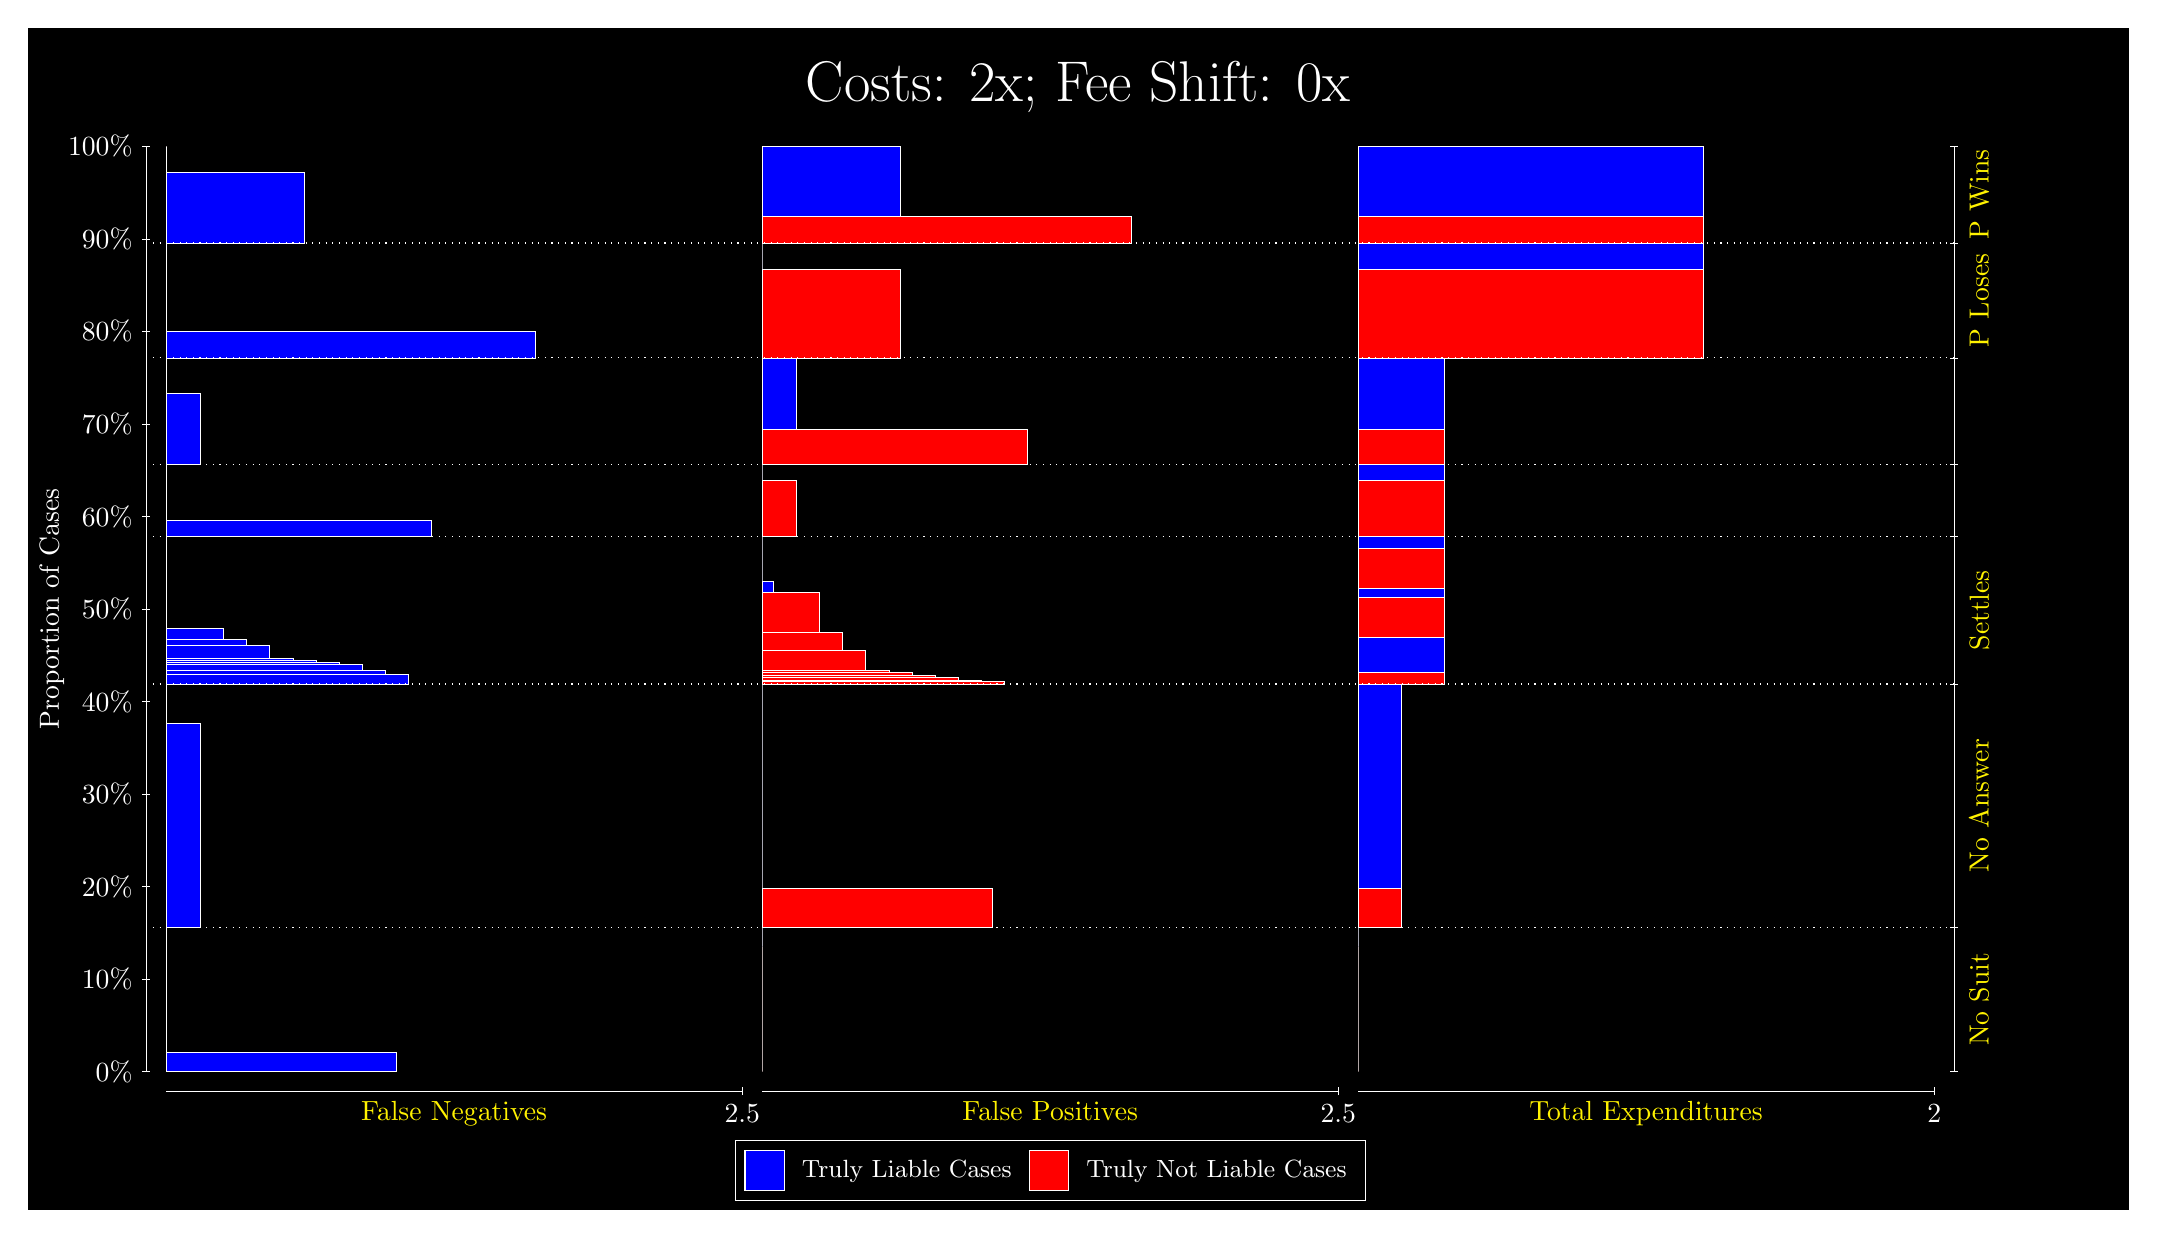
\begin{tikzpicture}
\draw[fill=black] (0,0) rectangle (26.667,15);
\draw[text=white] (0,13.5) rectangle (26.667,15) node[midway] {\huge Costs: 2x; Fee Shift: 0x};
\draw[white, very thin] (1.5,1.75) -- (1.5,13.5);
\node[rotate=90, text=white, anchor=center] at (0.3, 7.625) {Proportion of Cases};
\draw[white, very thin] (1.45,1.75) -- (1.55,1.75);
\node[text=white, anchor=east] at (1.45, 1.75) {0\%};
\draw[white, very thin] (1.45,2.925) -- (1.55,2.925);
\node[text=white, anchor=east] at (1.45, 2.925) {10\%};
\draw[white, very thin] (1.45,4.1) -- (1.55,4.1);
\node[text=white, anchor=east] at (1.45, 4.1) {20\%};
\draw[white, very thin] (1.45,5.275) -- (1.55,5.275);
\node[text=white, anchor=east] at (1.45, 5.275) {30\%};
\draw[white, very thin] (1.45,6.45) -- (1.55,6.45);
\node[text=white, anchor=east] at (1.45, 6.45) {40\%};
\draw[white, very thin] (1.45,7.625) -- (1.55,7.625);
\node[text=white, anchor=east] at (1.45, 7.625) {50\%};
\draw[white, very thin] (1.45,8.8) -- (1.55,8.8);
\node[text=white, anchor=east] at (1.45, 8.8) {60\%};
\draw[white, very thin] (1.45,9.975) -- (1.55,9.975);
\node[text=white, anchor=east] at (1.45, 9.975) {70\%};
\draw[white, very thin] (1.45,11.15) -- (1.55,11.15);
\node[text=white, anchor=east] at (1.45, 11.15) {80\%};
\draw[white, very thin] (1.45,12.325) -- (1.55,12.325);
\node[text=white, anchor=east] at (1.45, 12.325) {90\%};
\draw[white, very thin] (1.45,13.5) -- (1.55,13.5);
\node[text=white, anchor=east] at (1.45, 13.5) {100\%};

\draw[white, very thin] (24.457,1.75) -- (24.457,13.5);
\draw[white, very thin] (24.407,1.75) -- (24.507,1.75);
\node[anchor=west] at (24.407, 1.75) {};
\draw[white, very thin] (24.407,3.5819) -- (24.507,3.5819);
\node[anchor=west] at (24.407, 3.5819) {};
\draw[white, very thin] (24.407,6.672) -- (24.507,6.672);
\node[anchor=west] at (24.407, 6.672) {};
\draw[white, very thin] (24.407,8.5462) -- (24.507,8.5462);
\node[anchor=west] at (24.407, 8.5462) {};
\draw[white, very thin] (24.407,9.4594) -- (24.507,9.4594);
\node[anchor=west] at (24.407, 9.4594) {};
\draw[white, very thin] (24.407,10.813) -- (24.507,10.813);
\node[anchor=west] at (24.407, 10.813) {};
\draw[white, very thin] (24.407,12.272) -- (24.507,12.272);
\node[anchor=west] at (24.407, 12.272) {};
\draw[white, very thin] (24.407,13.5) -- (24.507,13.5);
\node[anchor=west] at (24.407, 13.5) {};

\draw[white, very thin, fill=blue] (1.75,1.75) rectangle (4.6775,1.9951);
\draw[white, very thin, fill=red] (1.75,1.9951) rectangle (1.75,3.5819);
\draw[white, very thin, fill=blue] (1.75,3.5819) rectangle (2.1891,6.1726);
\draw[white, very thin, fill=red] (1.75,6.1726) rectangle (1.75,6.672);
\draw[white, very thin, fill=blue] (1.75,6.672) rectangle (4.8239,6.79);
\draw[white, very thin, fill=blue] (1.75,6.79) rectangle (4.5312,6.8484);
\draw[white, very thin, fill=blue] (1.75,6.8484) rectangle (4.2384,6.9182);
\draw[white, very thin, fill=blue] (1.75,6.9182) rectangle (3.9457,6.9453);
\draw[white, very thin, fill=blue] (1.75,6.9453) rectangle (3.6529,6.9791);
\draw[white, very thin, fill=blue] (1.75,6.9791) rectangle (3.3602,6.9999);
\draw[white, very thin, fill=blue] (1.75,6.9999) rectangle (3.0674,7.1634);
\draw[white, very thin, fill=blue] (1.75,7.1634) rectangle (2.7746,7.2387);
\draw[white, very thin, fill=blue] (1.75,7.2387) rectangle (2.4819,7.3804);
\draw[white, very thin, fill=red] (1.75,7.3804) rectangle (1.75,8.5462);
\draw[white, very thin, fill=blue] (1.75,8.5462) rectangle (5.1167,8.746);
\draw[white, very thin, fill=red] (1.75,8.746) rectangle (1.75,9.4594);
\draw[white, very thin, fill=blue] (1.75,9.4594) rectangle (2.1891,10.362);
\draw[white, very thin, fill=red] (1.75,10.362) rectangle (1.75,10.813);
\draw[white, very thin, fill=blue] (1.75,10.813) rectangle (6.4341,11.149);
\draw[white, very thin, fill=red] (1.75,11.149) rectangle (1.75,12.272);
\draw[white, very thin, fill=blue] (1.75,12.272) rectangle (3.5065,13.165);
\draw[white, very thin, fill=red] (1.75,13.165) rectangle (1.75,13.5);
\draw[white, very thin, fill=red] (9.3189,1.75) rectangle (9.3189,3.3369);
\draw[white, very thin, fill=blue] (9.3189,3.3369) rectangle (9.3189,3.5819);
\draw[white, very thin, fill=red] (9.3189,3.5819) rectangle (12.246,4.0813);
\draw[white, very thin, fill=blue] (9.3189,4.0813) rectangle (9.3189,6.672);
\draw[white, very thin, fill=red] (9.3189,6.672) rectangle (12.393,6.704);
\draw[white, very thin, fill=red] (9.3189,6.704) rectangle (12.1,6.7219);
\draw[white, very thin, fill=red] (9.3189,6.7219) rectangle (11.807,6.7621);
\draw[white, very thin, fill=red] (9.3189,6.7621) rectangle (11.515,6.7818);
\draw[white, very thin, fill=red] (9.3189,6.7818) rectangle (11.222,6.8151);
\draw[white, very thin, fill=red] (9.3189,6.8151) rectangle (10.929,6.8249);
\draw[white, very thin, fill=red] (9.3189,6.8249) rectangle (10.929,6.8428);
\draw[white, very thin, fill=red] (9.3189,6.8428) rectangle (10.636,7.0955);
\draw[white, very thin, fill=red] (9.3189,7.0955) rectangle (10.344,7.3334);
\draw[white, very thin, fill=red] (9.3189,7.3334) rectangle (10.051,7.8378);
\draw[white, very thin, fill=blue] (9.3189,7.8378) rectangle (9.4652,7.9795);
\draw[white, very thin, fill=blue] (9.3189,7.9795) rectangle (9.3189,8.5462);
\draw[white, very thin, fill=red] (9.3189,8.5462) rectangle (9.758,9.2595);
\draw[white, very thin, fill=blue] (9.3189,9.2595) rectangle (9.3189,9.4594);
\draw[white, very thin, fill=red] (9.3189,9.4594) rectangle (12.686,9.9111);
\draw[white, very thin, fill=blue] (9.3189,9.9111) rectangle (9.758,10.813);
\draw[white, very thin, fill=red] (9.3189,10.813) rectangle (11.075,11.936);
\draw[white, very thin, fill=blue] (9.3189,11.936) rectangle (9.3189,12.272);
\draw[white, very thin, fill=red] (9.3189,12.272) rectangle (14.003,12.607);
\draw[white, very thin, fill=blue] (9.3189,12.607) rectangle (11.075,13.5);
\draw[white, very thin, fill=red] (16.888,1.75) rectangle (16.888,3.3369);
\draw[white, very thin, fill=blue] (16.888,3.3369) rectangle (16.888,3.5819);
\draw[white, very thin, fill=red] (16.888,3.5819) rectangle (17.437,4.0813);
\draw[white, very thin, fill=blue] (16.888,4.0813) rectangle (17.437,6.672);
\draw[white, very thin, fill=red] (16.888,6.672) rectangle (17.986,6.8249);
\draw[white, very thin, fill=blue] (16.888,6.8249) rectangle (17.986,7.27);
\draw[white, very thin, fill=red] (16.888,7.27) rectangle (17.986,7.7744);
\draw[white, very thin, fill=blue] (16.888,7.7744) rectangle (17.986,7.8924);
\draw[white, very thin, fill=red] (16.888,7.8924) rectangle (17.986,8.4009);
\draw[white, very thin, fill=blue] (16.888,8.4009) rectangle (17.986,8.5462);
\draw[white, very thin, fill=red] (16.888,8.5462) rectangle (17.986,9.2595);
\draw[white, very thin, fill=blue] (16.888,9.2595) rectangle (17.986,9.4594);
\draw[white, very thin, fill=red] (16.888,9.4594) rectangle (17.986,9.9111);
\draw[white, very thin, fill=blue] (16.888,9.9111) rectangle (17.986,10.813);
\draw[white, very thin, fill=red] (16.888,10.813) rectangle (21.279,11.936);
\draw[white, very thin, fill=blue] (16.888,11.936) rectangle (21.279,12.272);
\draw[white, very thin, fill=red] (16.888,12.272) rectangle (21.279,12.607);
\draw[white, very thin, fill=blue] (16.888,12.607) rectangle (21.279,13.5);
\draw[white, dotted] (1.5,3.5819) -- (24.457,3.5819);
\draw[white, dotted] (1.5,6.672) -- (24.457,6.672);
\draw[white, dotted] (1.5,8.5462) -- (24.457,8.5462);
\draw[white, dotted] (1.5,9.4594) -- (24.457,9.4594);
\draw[white, dotted] (1.5,10.813) -- (24.457,10.813);
\draw[white, dotted] (1.5,12.272) -- (24.457,12.272);
\draw[white, very thin] (1.75,1.5) -- (9.0689,1.5);
\node[text=yellow, anchor=north] at (5.4094, 1.5) {False Negatives};
\draw[white, very thin] (9.0689,1.45) -- (9.0689,1.55);
\node[text=white, anchor=north] at (9.0689, 1.45) {2.5};

\draw[white, very thin] (9.3189,1.5) -- (16.638,1.5);
\node[text=yellow, anchor=north] at (12.978, 1.5) {False Positives};
\draw[white, very thin] (16.638,1.45) -- (16.638,1.55);
\node[text=white, anchor=north] at (16.638, 1.45) {2.5};

\draw[white, very thin] (16.888,1.5) -- (24.207,1.5);
\node[text=yellow, anchor=north] at (20.547, 1.5) {Total Expenditures};
\draw[white, very thin] (24.207,1.45) -- (24.207,1.55);
\node[text=white, anchor=north] at (24.207, 1.45) {2};

\node[text=yellow, centered, rotate=90] at (24.777, 2.666) {No Suit};
\node[text=yellow, centered, rotate=90] at (24.777, 5.127) {No Answer};
\node[text=yellow, centered, rotate=90] at (24.777, 7.6091) {Settles};


\node[text=yellow, centered, rotate=90] at (24.777, 11.543) {P Loses};
\node[text=yellow, centered, rotate=90] at (24.777, 12.886) {P Wins};

\draw (12.978300999999998,1.5) node[draw=none] (baseCoordinate) {};
\begin{scope}[align=center]
        \matrix[scale=0.5, draw=white, below=0.5cm of baseCoordinate, nodes={draw}, column sep=0.1cm]{
            \node[rectangle, draw, minimum width=0.5cm, minimum height=0.5cm, fill=blue] {}; &
            \node[draw=none, font=\small, text=white] (B) {Truly Liable Cases}; &
            \node[rectangle, draw, minimum width=0.5cm, minimum height=0.5cm, fill=red] {}; &
            \node[draw=none, font=\small, text=white] (B) {Truly Not Liable Cases}; \\
            };
\end{scope}

\end{tikzpicture}
\end{document}